\documentclass[12pt]{extarticle}

%%%% paramètres généraux
%%%% french character
\usepackage[french]{babel}
\usepackage[T1]{fontenc}
\usepackage[utf8]{inputenc}

%%%% useful packages
\usepackage[a4paper, left=1.3cm, right=1.3cm, top=2.2cm, bottom=2.3cm]{geometry}
\usepackage{subcaption} % for figure caption
\usepackage{graphicx} % image
\usepackage{tabularx} % table
\usepackage{lastpage} %pour la définition de la dernière page
\usepackage[table]{xcolor} % color in table
\usepackage{amsmath} % math
\usepackage{amssymb} % bold math
\usepackage{wasysym} % integral
\usepackage[many]{tcolorbox} % colored box
\usepackage{awesomebox} % pour des box déjà définies
\usepackage{fancyhdr} % headers
\usepackage{enumitem} % for bullet in itemize
\usepackage[colorlinks=true,linkcolor=black,citecolor=black,filecolor=black,urlcolor=black]{hyperref} % for link
\usepackage[backend=biber,style=alphabetic,sorting=ynt]{biblatex}
\usepackage{accents} % for complex notation
\usepackage[european, straightvoltages, RPvoltages]{circuitikz} % for electronic circuit

\usepackage{hyperref}   %pour les liens url et les références
\hypersetup{
    colorlinks=true,
    urlcolor=blue,
    linkcolor=blue,
    breaklinks=true
}
\usepackage{empheq}
\usepackage{multicol} % to use several columns
%\setlength{\columnseprule}{1pt} %Separator ruler width
\usepackage{cellspace}  % espace du texte dans les colonnes tableaux
\usepackage{colortbl}  %pour colorier les cases de tableaux
\tcbuselibrary{skins} %library de 
\usepackage{shadow}
\usepackage{pifont}

\usepackage{fontawesome5}

%\usepackage{fontawesome} % awesome icons
\usepackage{ifthen} % for loop and boolean in commands
\usepackage{qrcode}
\usepackage{pdfpages} % to include pdf
\usepackage{wrapfig} % to wrap text around figures
\usepackage{chemfig} % to draw chemistry formula
\usepackage{chemist} % surtout pour chemform
\usepackage{multirow} % for vertically merged cells
\usepackage{makecell} % to format cell in tables
\usepackage{physics} % for derivatives, braket, etc.
\usepackage{esvect} % for large vectors
\usepackage{listings} % for code
\usepackage{dashundergaps} % for automatic text to fill
% dyslexia friendly font (need to be compiled in xetex)
%\usepackage{fontspec}
%\setmainfont{OpenDyslexic}
\usepackage{tikz}
\usepackage{pgfplots}
\usepackage[framemethod=tikz]{mdframed} %pour les boîtes
\usepackage{dashundergaps} %pour les textes à trous

%%%% settings
\setlength{\parskip}{0cm}
\setlength{\parindent}{0cm}
\renewcommand{\baselinestretch}{1.3}
\setcounter{tocdepth}{2}
\renewcommand{\thesection}{\textcolor{red}{\Roman{section}}}
\renewcommand{\thesubsection}{\textcolor{red}{\Roman{section}.\arabic{subsection}}}

%%%% tikz configuration
\usetikzlibrary{babel}
\tikzset{>=latex}
\usetikzlibrary{shadows}
\usetikzlibrary{backgrounds}



%%%% header
\renewcommand{\headrulewidth}{0.4pt}
\setlength{\headheight}{22.50113pt}


%%%% Table
\renewcommand{\tabularxcolumn}[1]{m{#1}}
\setlength{\extrarowheight}{8pt}
\newcolumntype{P}[1]{>{\centering\arraybackslash}p{#1\linewidth}}% colonne de type p mais centrée
\cellspacetoplimit 2pt %espace au dessus du texte
\cellspacebottomlimit 2pt  %espace en dessous du texte



%%%% Chemfig configuration
\setchemfig{
  atom sep=20pt,
  bond style={line width=1pt},
  angle increment=30
}


%%%% dashundergaps configuration
\dashundergapssetup{
  gap-numbers = false,
  gap-format = dot,
  gap-widen,
  gap-extend-percent
}


%\bibliographystyle{plain}
\bibliography{TSNR/TSNR.bib}

%%%% quelques commandes
%%%%%%%%%%%%%%%%%%%%%%%%%%%%%%%%%%%%%%%%%%%%%%%%%%%%%%%%%%%%%%%%%%%%%%%%%%
%%%% quelque couleurs
\definecolor{vertSombre} {RGB}{  0,  92,  46}
\definecolor{cyanSombre} {RGB}{  0, 140, 128}
\definecolor{jauneSombre}{RGB}{138, 103,   0}
\definecolor{jauneClair} {RGB}{218, 173,   0}
\definecolor{rougeSombre}{RGB}{148,  31,   0}
\definecolor{rougeClair} {RGB}{224,  39,  34}
\definecolor{couleurtitre}{RGB}{255,  255,  255}
\definecolor{exef}{RGB}{210,210,210}
\definecolor{propositiono}{RGB}{109,109,109}

%%% quelques couleurs dérivées des couleurs choisie
\newcommand{\couleurCorrection}{couleurPrincipale!60!black}
\newcommand{\couleurExercice}{couleurPrincipale!75!black}

%%%% rectangle coloré
\newcommand\rectangle[3]{%
  \shorthandoff{;}
  \tikz \node (rect) [draw, fill, color=#1,
              minimum width=#2,
              minimum height=#3] {};
  \shorthandon{;}
}
\newcommand\rectangleCyan[2]{\rectangle{couleurPrincipale}{#1}{#2}}

%%%% simple boite
\newenvironment{boite}{
  \begin{tcolorbox}
  [ breakable, enhanced jigsaw, % to break box over page
    arc = 0mm, % straight line
    colback= white, % white background
    colframe= black % dark frame
  ]
}
{ \end{tcolorbox} }

\newtcolorbox{facile}[2][]{colback=green!5!white,
colframe=green!75!black,fonttitle=\bfseries,
colbacktitle=green!85!black,enhanced,
attach boxed title to top center={yshift=-2mm},
title={#2},#1}

\newtcolorbox{difficile}[2][]{colback=red!5!white,
colframe=red!75!black,fonttitle=\bfseries,
colbacktitle=red!85!black,enhanced,
attach boxed title to top center={yshift=-2mm},
title={#2},#1}


%\newenvironment[1]{Propriete}{\begin{tcolorbox}[colback=red!5!white,colframe=red!75!black,title=\textbf{#1 :}]
%}
%{\end{tcolorbox} 


%%%%%%%%%%%%%%%%%%%%%%%%%%%%%%%%%%%%%%%%%%%%%%%%%%%%%%%%%%%%%%%%%%%%%%%%%%
%%%% pagination et sections
\newcommand{\titre}[1]{
  \begin{center}
    \textsf{\bfseries \Large #1}
  \end{center}
}
\newcommand{\sousTitre}[1]{
  \textsf{\bfseries #1}
}
\newcommand{\pasDePagination}{
  \thispagestyle{empty}
}
\newcommand{\feuilleBlanche}{
  \newpage
  \phantom{b}
  \pasDePagination
}


%%%% activité ou TP
\newcounter{acti}
\newcommand{\titreActi}[2]{
  \refstepcounter{acti}
  \titre{#1 \arabic{section}.\arabic{acti} -- #2}
}
\newcommand{\titreTP}[1]{
  \titreActi{TP}{#1}
  %\titreActi{Activité expérimentale}{#1}
}
\newcommand{\titreActivite}[1]{
  \titreActi{Activité}{#1}
}
\newcommand{\titreEvaluation}[1]{
  \titreActi{Évaluation}{#1}
}


%%%% chapitre, section et sous-section
\newcommand{\titreChapitre}[1]{
  \titre{Chapitre \arabic{section} : #1}
}
\newcommand{\titrePartie}[1]{
  \vspace*{24pt}
  \refstepcounter{subsection}
  \rectangleCyan{60pt}{1pt}
  \sousTitre{\Large \Roman{subsection} -- #1}
  \rectangleCyan{60pt}{1pt}
  \vspace*{10pt}
}
\newcounter{sousSection}
\newcommand{\titreSection}[1]{
  \vspace*{16pt}
  \refstepcounter{subsubsection}
  \setcounter{sousSection}{0}
  \rectangleCyan{30pt}{4pt}
  \sousTitre{\large \arabic{subsubsection} -- #1}
  \vspace*{10pt}
}
\newcommand{\titreSousSection}[1]{
  \vspace*{12pt}
  \refstepcounter{sousSection}
  \sousTitre{\Alph{sousSection} -- #1}
  \vspace*{8pt}
}

%%%% fixe le numéro de l'activité
\newcommand{\numeroActivite}[1]{
  \setcounter{subsection}{0}
  \setcounter{subsubsection}{0}
  \setcounter{sousSection}{0}
  \setcounter{figure}{0}
  \setcounter{document}{0}
  \setcounter{exercice}{0}
  \setcounter{QCM}{0}
  \setcounter{countCoupDePouce}{0}
  \setcounter{acti}{#1 - 1}
  \setcounter{page}{1}
}
% fixe le numéro de page (#2) et de partie (#1)
\newcommand{\numeroPartieCours}[2]{
  \newpage
  \setcounter{subsection}{#1 - 1}
  \setcounter{page}{#2}
}

%%%% lignes
\newcommand{\ligne}{
  \par\noindent\rule{\textwidth}{0.4pt}
}
\newcommand{\lignePointillee}[1]{
  \makebox[#1\textwidth]{\dotfill}
}


%%%%%%%%%%%%%%%%%%%%%%%%%%%%%%%%%%%%%%%%%%%%%%%%%%%%%%%%%%%%%%%%%%%%%%%%%%
%%%% en-tête
\newcommand{\teteGauche}[1]{
  \lhead{
    \textbf{\footnotesize #1}
  }
}
\newcommand{\teteDroite}[1]{
  \rhead{
    \hfill \textbf{\footnotesize #1}
  }
}

%

\newcommand{\enTeteRevision}[2]{
  \pagestyle{fancy}
  \lhead{Revision #1 - \textit{#2}}
  %\chead{} % central header
  \teteDroite{Lycée Parc de Vilgénis 2023 - 2024}
}

\newcommand{\enTeteExercice}[1]{
  \pagestyle{fancy}
  \lhead{Exercices du Chapitre #1}
  %\chead{} % central header
  \teteDroite{Lycée Parc de Vilgénis 2023 - 2024}
}

\newcommand{\enTeteMethodo}[2]{
  \pagestyle{fancy}
  \teteGauche{Fiche Méthode #1 : #2}
  %\chead{} % central header
  \teteDroite{Lycée Parc de Vilgénis 2023 - 2024}
}

\newcommand{\enTeteChap}[2]{
  \pagestyle{fancy}
  \lhead{Chapitre #1 - \textit{#2}}
  %\chead{} % central header
  \teteDroite{Lycée Parc de Vilgénis 2023 - 2024}
}

\newcommand{\enTeteExo}[1]{
  \pagestyle{fancy}
  \lhead{Exercices du Chapitre #1}
  %\chead{} % central header
  \teteDroite{Lycée Parc de Vilgénis 2023 - 2024}
}

\newcommand{\enTeteAct}[3]{
  \pagestyle{fancy}
  \lhead{Chapitre #1 \newline Activité #2 - \textit{#3}}
  %\chead{} % central header
  \teteDroite{Lycée Parc de Vilgénis 2023 - 2024}
}

\newcommand{\enTeteDM}[2]{
  \pagestyle{fancy}
  \lhead{Devoir Maison n$\degree$ #1 - \textit{#2}}
  %\chead{} % central header
  \teteDroite{Lycée Parc de Vilgénis 2023 - 2024}
}

\newcommand{\enTeteTP}[2]{
  \pagestyle{fancy}
  \lhead{TP #1 - \textit{#2}}
  %\chead{} % central header
  \teteDroite{Lycée Parc de Vilgénis 2023 - 2024}
}
%
\newcommand{\enTeteSeance}[2]{
  \pagestyle{fancy}
  \lhead{Date : \textit{#1}}
  \chead{Séance : #2}
  \teteDroite{Seconde} % central header
}
%

\newcommand{\enTeteFicheReussite}[1]{
  \newpage
  \setcounter{subsection}{0}
  \pasDePagination
  
  \phantom{b}
  \vspace*{-70pt}
  \titre{Fiche \og Réussir son évaluation \fg}
  \titre{#1}
  
  \vspace*{-6pt}
  % \titreSection{Ce que je dois savoir}
  
  Pour savoir quoi réviser, je lis les points clés du chapitre évalués :
  \begin{itemize}
    \item Si je pense maîtriser une notion, je coche la case \ok
    \item Si je pense que je dois la retravailler, je coche la case \pasOk
  \end{itemize}
  
  Pour travailler les notions qui ne sont pas maîtrisées, je reprend les activités associés.
}
\newcommand{\basDePageFicheReussite}{
  \titreSection{Ce qu'il me reste à faire}
}
\newcommand{\travailExerciceCorrige}{
  Pour être sûr-e d'obtenir une bonne note, je m'entraîne avec les exercices corrigés du manuel indiqués dans la colonne de droite.
}
\newcommand{\questionFicheReussite}[1]{
  S'il me reste des questions, je les note ici pour les poser au début de l'évaluation :\\[4pt]
  \lignesReponse{#1}
}
\newcommand{\coursFicheReussite}{
  Je prépare une fiche au format A4 avec toutes les notions, définitions ou grandeurs dont je pense avoir besoin pendant l'évaluation.
}


%%%%%%%%%%%%%%%%%%%%%%%%%%%%%%%%%%%%%%%%%%%%%%%%%%%%%%%%%%%%%%%%%%%%%%%%%%
%%%% exercice
% définit un booléen pour entrer ou sortir du mode correction
\newboolean{modeProf}
\setboolean{modeProf}{false}
\newcommand{\modeCorrection}{
  \setboolean{modeProf}{true}
  \TeacherModeOn
}

% définit une commande pour afficher une question 
% #1 : question
% #2 : réponse
% #3 : nombres de lignes pour répondre
\newcommand{\question}[3]{
  \numeroQuestion\!#1
  
  % pointille ou correction
  \ifthenelse {\boolean{modeProf}} { % prof
    \reponseCorrigee{#2}
  }{ % eleve
    \vspace*{8pt}
    \lignesReponse{#3}
  }
}

%
\newcounter{exercice}
\newcommand{\numeroQuestion}{
  \refstepcounter{exercice}
  \vspace*{2pt}
  \hspace{15pt}
  \textcolor{black}{%couleurPrincipale!75!black}{
    \textbf{\arabic{exercice}} {\small\faMinus}
  }
}

% correction
\newcommand{\reponseCorrigee}[1]{
  \vspace*{2pt}
  \hspace{16pt}
  \textcolor{red}{
    \faCaretRight \hspace{2pt} #1
  }
}
\newcommand{\correction}[1]{
  \ifthenelse {\boolean{modeProf}} { % prof
    \textcolor{red}{#1}
  }{ % eleve
  }
}

% trace des lignes pour répondre
\newcounter{int}
\newcommand{\lignesReponse}[1]{
  \setcounter{int}{-1}
  \loop
    \stepcounter{int}
    \ifnum \value{int} < #1
    \lignePointillee{0.99} \\[8pt]
  \repeat
  \ifnum #1 > 0
    \vspace*{-12pt}
  \fi
}

% sous questions
\newcommand{\sousQuestion}[2]{
  \hspace{15pt}
  \textcolor{couleurPrincipale!75!black}{\textbullet} #1
  
  \vspace*{8pt}
  \reponse{#2}
}


%%%%%%%%%%%%%%%%%%%%%%%%%%%%%%%%%%%%%%%%%%%%%%%%%%%%%%%%%%%%%%%%%%%%%%%%%%
%%%% QCM
% question QCM
\newcounter{QCM}
\newcommand{\QCM}[2]{
  \refstepcounter{QCM}
  \vspace*{2pt}
  \textcolor{couleurPrincipale!75!black}{\textbf{\arabic{QCM}} {\small\faMinus}} #1
  
  \begin{qcm}
    #2
  \end{qcm}
}


%%%% Pour afficher les compétences
\newcommand{\competence}[1]{
  ~{\footnotesize\textit{(#1)}}
}


%%%% Espace pour indiquer nom, prénom et classe
\newcommand{\nomPrenomClasse}{
  \vspace*{-24pt}
  \underline{Nom} : \lignePointillee{0.3}\hfill \underline{Date } : \gap{....}/\gap{....}/\gap{....} \newline 
  \underline{Prénom} : \lignePointillee{0.3} \hfill\underline{Classe} : \gap{........}
}


%%%%%%%%%%%%%%%%%%%%%%%%%%%%%%%%%%%%%%%%%%%%%%%%%%%%%%%%%%%%%%%%%%%%%%%%%%
% texte à trou automatique
\newcommand{\texteTrouAuto}[1]{
  \gap{
    \textcolor{couleurPrincipale!60!black}{ \textbf{#1} }
  }
}

% texte à trou dans une ligne réglable
\newcommand{\texteTrou}[2]{
  \ifthenelse {\boolean{modeProf}} {% prof
    \textcolor{couleurPrincipale!60!black}{ \textbf{#1} }
  }{% élève
    \espaceReponse
    \lignePointillee{#2}
  }
}

% texte à trou sur plusieurs lignes
\newcommand{\texteTrouLigneComplete}[1]{
  \ifthenelse {\boolean{modeProf}} {% prof
    \textcolor{couleurPrincipale!60!black}{ \textbf{#1} }
  }{% élève
    \espaceReponse \dotfill
  }
}

% texte à trou sur plusieurs lignes
\newcommand{\texteTrouMultiLignes}[2]{
  \ifthenelse {\boolean{modeProf}} {% prof
    \textcolor{couleurPrincipale!60!black}{ \textbf{#1} }
  }{% élève
    \reponseLigne
    \lignesReponse{#2}
  }
}

% reponse en fin de ligne
\newcommand{\reponseLigne}{
  \espaceReponse
  \dotfill \\[8pt]
}

% espace vertical pour la réponse
\newcommand{\espaceReponse}{
  \phantom{$\Frac{1}{1}$} % espace vertical
  \hspace*{-40pt} \phantom{b} % ajuste l'espace horizontal
}

%%%%%%%%%%%%%%%%%%%%%%%%%%%%%%%%%%%%%%%%%%%%%%%%%%%%%%%%%%%%%%%%%%%%%%%%%%
%%%% Pour choisir parmi deux sujets
\newboolean{sujetA}
\setboolean{sujetA}{true}
\newcommand{\sujetB}{
  \setboolean{sujetA}{false}
}
\newcommand{\sujetA}{
  \setboolean{sujetA}{true}
}

%%%% Pour faire plusieurs sujets en parallèle
\newcommand{\variationSujet}[2]{
  \ifthenelse {\boolean{sujetA}}
  {\hspace*{-2pt}#1\hspace*{-2pt}}
  {\hspace*{-2pt}#2\hspace*{-2pt}}
}


%%%%%%%%%%%%%%%%%%%%%%%%%%%%%%%%%%%%%%%%%%%%%%%%%%%%%%%%%%%%%%%%%%%%%%%%%%
%%%% documents
\newcounter{document}
\newcommand{\titreDocu}[1]{
  \refstepcounter{document} % update counter
  \textbf{Document \arabic{document} -- #1} % print document title
  \addcontentsline{toc}{document}{\protect\numberline{} #1} % update table of content
}
\newenvironment{doc}[1]{
  \begin{boite}
    \titreDocu {#1} \newline
}
{ \end{boite} }

%\newenvironment{exo}[1]{
%\begin{mdframed}[style=autreexo]
%\textbf{\bsc{Exercice de cours 1} - Espèces chimiques}\\
%Donner le type (\textit{atomique}, \textit{moléculaire} ou \textit{ionique}) des espèces chimiques suivantes : hélium (He), eau (H\textsubscript{2}O), chlorure de sodium (Na$^{+}$, Cl$^{-}$).
%\end{mdframed}
%}
%% pour les référencer
\newcommand{\docu}[1]{
  \textbf{(Doc. #1)}
}


%%%% problematique
\newcommand{\problematique}[1]{
  %\hspace{8pt}
  \noindent\textcolor{red}{\begin{large} \textbf{\underline{Problématique} : }\end{large}}\textbf{#1}
  }



%%%% objectifs
\newenvironment{objBoite}{
  \begin{tcolorbox}
  [boxrule = 0pt,
  frame hidden, sharp corners,
  colback = white, enhanced,
  borderline north={2pt}{0pt}{couleurPrincipale},
  borderline south={2pt}{0pt}{couleurPrincipale},
  borderline west={4pt}{0pt}{couleurPrincipale},
  borderline east={4pt}{0pt}{couleurPrincipale}
  ]
  
}
{
  \end{tcolorbox}
}
\newenvironment{objectifs}{
  \begin{objBoite}
    \begin{center}
      \sousTitre{\large Objectifs de la séance :}
      \begin{listeObjectifs}
}
{ 
      \end{listeObjectifs}
    \end{center}
  \end{objBoite}
}

%%%% Espace pour un coup de pouce
\newcounter{countCoupDePouce}
\newenvironment{coupDePouce}{
  \refstepcounter{countCoupDePouce}
  \vspace*{-12pt}
  \begin{boite}
    \begin{flushright}
      \textcolor{couleurPrincipale}{\faSquareO}
    \end{flushright}
    
    \vspace*{-30pt}
    \textcolor{couleurPrincipale}{\faThumbsUp}
    \textbf{Coup de pouce \arabic{countCoupDePouce}} :\\[4pt]
}
{
  \end{boite}
}


%%%% Espace pour une appréciation
\newcommand{\appreciation}[1]{
  \vspace*{8pt}
  \sousTitre{Appréciation et remarques}
  \vspace*{-8pt}
  \begin{boite}
    \vspace{#1 pt}
    \phantom{b}
  \end{boite}
}


%%%%%%%%%%%%%%%%%%%%%%%%%%%%%%%%%%%%%%%%%%%%%%%%%%%%%%%%%%%%%%%%%%%%%%%%%%
%%%% Définit un nouveau type de colonne : taille fixée par une fraction
%%%% de la largeur de la ligne, avec un texte centré
\newcolumntype{C}[1]{>{\centering\arraybackslash}p{#1\linewidth}}

%%%% Tableau de competence
\newenvironment{tableauCompetences}{
  \centering
  \setlength{\extrarowheight}{6pt}
  \tabularx{\linewidth}{| c | X | c | c | c | c |}
    \hline
    \rowcolor{blue!25}
    \centering \textbf{Compétences} & \centering \textbf{Items} & \textbf{D} & \textbf{C} & \textbf{B} & \textbf{A}
    \\ \hline
}
{
    \\ \hline
  \endtabularx
}

%%%% Tableau de connaissances
\newenvironment{tableauConnaissances}{
  \centering
  \setlength{\extrarowheight}{6pt}
  \tabularx{\linewidth}{| X | c | c | C{0.18} | C{0.15} |}
    \hline
    \rowcolor{gray!20} 
    \textbf{Points clés du chapitre} & \ok & \pasOk & \textbf{En classe} & \textbf{Exercices}
    \\ \hline
}
{   
    \\ \hline
  \endtabularx
}

%%%% Tableau de connaissances sans exercices
\newenvironment{tableauConnaissancesSansExercices}{
  \centering
  \setlength{\extrarowheight}{6pt}
  \tabularx{\linewidth}{| X | c | c | C{0.2} |}
    \hline
    \rowcolor{gray!20} 
    \textbf{Points clés du chapitre} & \ok & \pasOk & \textbf{En classe}
    \\ \hline
}
{   
    \\ \hline
  \endtabularx
}

%%%% Tableau de correction élève
\newcommand{\correctionEleve}[1]{
  \setlength{\extrarowheight}{6pt}
  \begin{tabularx}{\linewidth}{| X | C{0.26} | C{0.26} | C{0.26} |}
    \hline
    \rowcolor{gray!20}
    \textbf{Question} &
    \textbf{L'erreur} &
    \textbf{Analyse de l'erreur} &
    \textbf{La correction}
    \\ \hline
    %
    \phantom{b} \vspace{#1 pt}
    & & & \\ \hline
    \phantom{b} \vspace{#1 pt}
    & & & \\ \hline
    \phantom{b} \vspace{#1 pt}
    & & & \\ \hline
    \phantom{b} \vspace{#1 pt}
    & & & \\ \hline
  \end{tabularx}
}

%%%% Tableau bilan de la correction
\newcommand{\bilanCorrection}[1]{
  \setlength{\extrarowheight}{6pt}
  \begin{tabularx}{\linewidth}{| X | X |}
    \hline
    \rowcolor{gray!20}
    \textbf{Ce que je n'avais pas compris...} &
    \textbf{Ce que maintenant j'ai compris...}
    \\ \hline
    \phantom{b} \vspace{#1 pt} % \newline \newline \newline
    & \\ \hline
  \end{tabularx}
}


%%%%%%%%%%%%%%%%%%%%%%%%%%%%%%%%%%%%%%%%%%%%%%%%%%%%%%%%%%%%%%%%%%%%%%%%%%
%%%% symboles : chevron, flèche, attention, etc.
\newcommand{\chevron}{
  \textcolor{couleurPrincipale}{\small \faChevronRight}
}
%
\newcommand{\fleche}{
  \textcolor{couleurPrincipale}{\faCaretRight}
}
%
\newcommand{\attention}{
  \textcolor{couleurPrincipale}{\faExclamationTriangle}
}
%
\newcommand{\flecheLongue}{
  \textcolor{red}{\longrightarrow}
}
%
\newcommand{\ok}{
  \textcolor{couleurPrincipale}{\faCheckCircle}
}
%
\newcommand{\pasOk}{
  \textcolor{couleurPrincipale}{\faTimesCircle}
}
%
\newcommand{\pointCyan}{
  \textcolor{couleurPrincipale}{\textbullet}
}
%
\newcommand{\mesure}{
  \hspace{15pt}
  \textcolor{couleurPrincipale!75!black}{\faWrench\faFlask}
}


%%%%%%%%%%%%%%%%%%%%%%%%%%%%%%%%%%%%%%%%%%%%%%%%%%%%%%%%%%%%%%%%%%%%%%%%%%
%%%% Passage important
\newenvironment{definition}[1]{
  \begin{tcolorbox}[colback=green!5!white,colframe=green!75!black,title=\textbf{#1}]
  
}
{
  \end{tcolorbox}
}

%%%% contexte
\newenvironment{contexte}{
  \begin{tcolorbox}
  [boxrule = 4pt, sharp corners,
  colframe = couleurPrincipale,
  colback = white!95!couleurPrincipale, % background color
  breakable, enhanced jigsaw] % to break box over page
  
}
{
  \end{tcolorbox}
}


%%%% emphase
\newcommand{\emphase}[1]{
  \textcolor{couleurImportant}{\textsf{\bfseries \large #1}}
}
%
\newcommand{\important}[1]{
  \!\textcolor{green}{\textbf{\bfseries #1}}\!\!
}
%
\newcommand{\exemple}{
  \flecheLongue \textit{Exemple :}
}
\newcommand{\exemples}{
  \flecheLongue \textit{Exemples :}
}
%
\newcommand{\note}{
  \textbf{Note :}
}
%
\newcounter{appelProf}
\newcommand{\appelProf}{
  \refstepcounter{appelProf}
  \hspace{24pt} \faHandPaperO \hspace{2pt}
  \textbf{Appel n$^\circ$ \arabic{appelProf} :}
}


%%%% image
\newcommand{\image}[2]{
  \includegraphics[width=#1\linewidth]{#2}
}


%%%%%%%%%%%%%%%%%%%%%%%%%%%%%%%%%%%%%%%%%%%%%%%%%%%%%%%%%%%%%%%%%%%%%%%%%%
%%%% qcm
\newlist{qcm}{itemize}{2}
\setlist[qcm]{label=$\square$, leftmargin=2cm}


%%%% liste d'objectif
\newlist{listeObjectifs}{itemize}{2}
\setlist[listeObjectifs]{label = \chevron}


%%%% protocole
\newlist{protocole}{itemize}{2}
\setlist[protocole]{label = {\footnotesize \fleche}}


%%%% liste de points
\newlist{listePoints}{itemize}{2}
\setlist[listePoints]{label = \pointCyan}


%%%% jeu de données
\newenvironment{donnees}{
  \textbf{Données :}
  \begin{listePoints}
}{
  \end{listePoints}
}


%%%% liste avec chiffre
\newlist{enumeration}{enumerate}{2}
\setlist[enumeration]{label = \textcolor{couleurPrincipale!75!black}{\textbf{\arabic*.}} }


%%%%%%%%%%%%%%%%%%%%%%%%%%%%%%%%%%%%%%%%%%%%%%%%%%%%%%%%%%%%%%%%%%%%%%%%%%
%%%% Séparation de la page
\newcommand{\separationTroisBlocs}[3]{
  \begin{minipage}[t]{0.3\linewidth}
    #1
  \end{minipage}
  ~
  \begin{minipage}[t]{0.3\linewidth}
    #2
  \end{minipage}
  ~
  \begin{minipage}[t]{0.3\linewidth}
    #3
  \end{minipage}
}
%%%%
\newcommand{\separationDeuxBlocs}[2]{
  \begin{minipage}[t]{0.48\linewidth}
    #1
  \end{minipage}
  \hfill
  \begin{minipage}[t]{0.48\linewidth}
    #2
  \end{minipage}
}
\newcommand{\separationBlocs}[4]{
  \begin{minipage}[t]{#1\linewidth}
    #3
  \end{minipage}
  \hfill
  \begin{minipage}[t]{#2\linewidth}
    #4
  \end{minipage}
}


%%%%%%%%%%%%%%%%%%%%%%%%%%%%%%%%%%%%%%%%%%%%%%%%%%%%%%%%%%%%%
%%%% tikz macros
%%%% rectangle
\newcommand{\tkzRect}[4]{
  \fill[color=#1] (#2,#4) -- (-#2,#4) -- (-#2,#3) -- (#2,#3);
}
\newcommand{\tkzEllipse}[4]{
  \fill[color=#1] (0,#3) ellipse (#2 and #4);
}
\newcommand{\tkzLegende}[4]{
  \draw[black, ->, very thick] (#2 + #4, #3) node[right] {#1} -- (#2, #3);
}
\newcommand{\tkzCercle}[4]{
  \filldraw [#3] (#1, #2) circle (#4pt);
}
\newcommand{\tkzCercleLigne}[5]{
  \filldraw [color = #4, fill = #3, very thick] (#1, #2) circle (#5pt);
}
%%%% tube à essais
\newcommand{\tkzTubeEssai}[3]{
  \draw[thick] (#1,#2) -- (#1,0) arc (0:-180:#1) -- (-#1,#2);
  \draw[thick] (0,#2) ellipse (#1 and #3);
}
\newcommand{\tkzBasTubeEssai}[5]{
  \fill[color=#1] (-#2,#3) -- (#2,#3) arc (0:-180:#2);
  \tkzRect{#1}{#2}{#3 - 0.01}{#4}
  \tkzEllipse{#1!85!black}{#2}{#4}{#5}
}
\newcommand{\tkzPhaseTubeEssai}[5]{
  \tkzRect{#1}{#2}{#3}{#4}
  \tkzEllipse{#1}{#2}{#3}{#5}
  \tkzEllipse{#1!85!black}{#2}{#4}{#5}
}

%%%% Point et vecteurs
\newcommand{\tkzLabel}[3]{
  \node at (#1, #2) {#3};
}
\newcommand{\tkzPointLabel}[3]{
  \filldraw (#1, #2) circle (2pt) node[above] {#3};
}
\newcommand{\tkzVecteur}[6]{
  \draw[black, ->, very thick] (#1, #2) -- (#1 + #3, #2 + #4) node[#6] {#5};
}
\newcommand{\tkzEquiv}[6]{
  \draw[black, <->, thick] (#1, #2) -- (#1 + #3, #2 + #4);
  \draw[black] (#1 + #3/2, #2 + #4/2) node[#6] {#5};
}
\newcommand{\tkzVecteurX}[4]{
  \draw[black, ->, very thick] (#1, #2) -- (#1 + #3, #2) node[above] {#4};
}
\newcommand{\tkzVecteurY}[4]{
  \draw[black, ->, very thick] (#1, #2) -- (#1, #2 + #3) node[right] {#4};
}
\newcommand{\tkzEquivY}[5]{
  \draw[#1, <->, thick] (#2, #3) -- (#2, #3 + #4);
  \draw[#1] (#2, #3 + #4/2) node[right] {#5};
}
\newcommand{\tkzEquivX}[5]{
  \draw[#1, <->, thick] (#2, #3) -- (#2 + #4, #3);
  \draw[#1] (#2 + #4/2, #3) node[below] {#5};
}

%%%% plan de classe
\newcommand{\rectangleTexte}[5]{
  \filldraw [fill=white, draw=black, ultra thick] (#1, #2) rectangle (#1 + #3, #2 + #4);
  \node at (#1 + #3/2, #2 + #4/2) [font=\sffamily] {\textbf{\large #5}};
}
% place dans la classe
\newcommand{\place}[3]{
  \rectangleTexte{#1}{#2}{3}{2}{#3}
}
\newcommand{\deuxPlaces}[4]{
  \place{#1}{#2}{#3}
  \place{#1 + 3}{#2}{#4}
}
\newcommand{\troisPlaces}[5]{
  \place{#1}{#2}{#3}
  \place{#1 + 3}{#2}{#4}
  \place{#1 + 6}{#2}{#5}
}
\newcommand{\quatrePlaces}[6]{
  \place{#1}{#2}{#3}
  \place{#1 + 3}{#2}{#4}
  \place{#1 + 6}{#2}{#5}
  \place{#1 + 9}{#2}{#6}
}
%%%% rangée
\newboolean{quatrePlace}
\setboolean{quatrePlace}{false}
\newcommand{\avecQuatrePlaces}{ \setboolean{quatrePlace}{true} }
\newcommand{\avecTroisPlaces}{ \setboolean{quatrePlace}{false} }
\newcommand{\rangee}[9]{
  \ifthenelse {\boolean{quatrePlace}} {
    \deuxPlaces  {0}{#1} {#2}{#3}
    \quatrePlaces{7}{#1} {#4}{#5}{#6}{#7}
    \deuxPlaces  {20}{#1}{#8}{#9}
  }{
    \deuxPlaces {#1}{#2}     {#3}{#4}
    \troisPlaces{#1 + 7}{#2} {#5}{#6}{#7}
    \deuxPlaces {#1 + 17}{#2}{#8}{#9}
  }
}
\newcommand{\rang}[9]{
  \ifthenelse {\boolean{quatrePlace}} {
    \deuxPlaces  {0} {12 - 3*#1} {#2}{#3}
    \quatrePlaces{7} {12 - 3*#1} {#4}{#5}{#6}{#7}
    \deuxPlaces  {20}{12 - 3*#1} {#8}{#9}
  }{
    \deuxPlaces {0} {12 - 3*#1} {#2}{#3}
    \troisPlaces{7} {12 - 3*#1} {#4}{#5}{#6}
    \deuxPlaces {17}{12 - 3*#1} {#7}{#8}
  }
}

%%%% TP
\newcommand{\paillasse}[3]{
  \rectangleTexte{#1}{#2}{4}{2}{#3}
}
\newcommand{\rangeeTP}[6]{
  \paillasse{#1}{#2}     {#3}
  \paillasse{#1 + 4}{#2} {#4}
  \paillasse{#1 + 12}{#2}{#5}
  \paillasse{#1 + 16}{#2}{#6}
}


%%%%%%%%%%%%%%%%%%%%%%%%%%%%%%%%%%%%%%%%%%%%%%%%%%%%%%%%%%%%%%%%%%%%%%%%%%
%%%% unité, degré, vecteur, etc.
\newcommand{\unit}[1]{
  \; \mathrm{#1}
}
\newcommand{\unitb}[1]{
  \unit{\mathbf{#1}}
}
\newcommand{\degree}{
  ^\circ\!
}
\newcommand{\degreCelsius}{
  \degree\, \mathrm{C}
}
\newcommand{\Frac}[2]{
  \displaystyle \frac{#1}{#2}
}
\newcommand{\algebrique}[1]{
  \overline{\mathrm{#1}}
}
\newcommand{\reaction}{
  \!\!\schemestart \arrow(.mid east--.mid west){->}[, 0.9, ultra thick] \schemestop\!\!
}
\newcommand{\metreParSeconde}{
  \unit{m\cdot s}^{-1}
}
%% grandeurs
\newcommand{\gISS}{g_\text{ISS}}
\newcommand{\MTerre}{M_\text{Terre}}
\newcommand{\RTerre}{R_\text{Terre}}
\newcommand{\inertie}{\text{inertie}}
\newcommand{\Tfus}{ T_{\text{f}} }
\newcommand{\Teb}{ T_{\text{éb}} }
\newcommand{\avogadro}{6,\!02 \times 10^{23}}
\newcommand{\saccha}{Saccharose (\chemfig{C_{12} H_{22} O_{11}})}
\newcommand{\vitamC}{Vitamine C (\chemfig{C_{6} H_{8} O_{6}})}
\newcommand{\ionsCa}{Ion calcium (\chemfig{Ca^{2+}})}
%% vecteurs
\newcommand{\FBsurA}{
  F_{B/A}
}
\newcommand{\FAsurB}{
  F_{A/B}
}
\newcommand{\vvFAsurB}{
  \vv{F}_{A/B}
}
\newcommand{\vvFBsurA}{
  \vv{F}_{B/A}
}

%% atome et isotope
\makeatletter
\newcommand{\isotope}[3]{%
   \settowidth\@tempdimb{\ensuremath{\scriptstyle#1}}%
   \settowidth\@tempdimc{\ensuremath{\scriptstyle#2}}%
   \ifnum\@tempdimb>\@tempdimc%
       \setlength{\@tempdima}{\@tempdimb}%
   \else%
       \setlength{\@tempdima}{\@tempdimc}%
   \fi%
  \begingroup%
  \ensuremath{
    ^{\makebox[\@tempdima][r]{\ensuremath{\scriptstyle#1}}}
    _{\makebox[\@tempdima][r]{\ensuremath{\scriptstyle#2}}}
    \chemfig{#3}
  }%
  \endgroup%
}%
\makeatother
%% element chimique
\makeatletter
\newcommand{\element}[2]{%
   \settowidth\@tempdimb{\ensuremath{\footnotesize #1}}%
  \begingroup%
  \ensuremath{
    _{\makebox[\@tempdimb][r]{\ensuremath{\small #1}}} 
    \chemfig[atom style={scale=1.3}]{#2}
  }%
  \endgroup%
}%
\makeatother

%% siècle
\newcommand{\siecle}[1]{
  \textsc{\romannumeral #1}\textsuperscript{e}~siècle
}
%% texte avec une boite autour
\newcommand{\texteEncadre}[1]{
  \frame{\vphantom{$\Frac{1}{10}$} \text{ #1 } }
}


%% papier millimétré
\newcommand{\papiermillimetre}{
\begin{tikzpicture}
	% Dimensions du repere
	\def\xmin{0} \def\xmax{18} \def\ymin{0} \def\ymax{25}
	% Grilles
	\draw [step=0.1cm,gray,ultra thin]  (\xmin,\ymin) grid (\xmax,\ymax);
	\draw [step=0.5cm,gray, thin] (\xmin,\ymin) grid (\xmax,\ymax);
	\draw [step=1cm,gray, thick] (\xmin,\ymin) grid (\xmax,\ymax);
	\draw [step=5cm,gray,very thick] (\xmin,\ymin) grid (\xmax,\ymax);
\end{tikzpicture}
}


%%%%%%%%%%%%%%%%%%%%%%%%%%%%%%%%%%%%%%%%%%%%%%%%%%%%%%%%%%%%%%%%%%%%%%%%%%
%%%% Couleur pour le code
\definecolor{vertCode}    {rgb}{0.2,0.6,0}
\definecolor{grisCode}    {rgb}{0.5,0.5,0.5}
\definecolor{violetCode}  {rgb}{0.58,0,0.82}
\definecolor{fondCode}    {rgb}{0.95,0.95,0.92}
%%%% Style python
\lstdefinestyle{codePython}{
    backgroundcolor=\color{fondCode},
    commentstyle=\color{magenta},
    keywordstyle=\color{vertCode},
    numberstyle=\tiny\color{grisCode},
    stringstyle=\color{violetCode},
    basicstyle=\ttfamily\footnotesize,
    breakatwhitespace=false,
    breaklines=true,
    captionpos=b,
    keepspaces=true,
    numbers=left,
    numbersep=5pt, 
    showspaces=false,
    showstringspaces=false,
    showtabs=false, 
    tabsize=2
}
\def\inline{\lstinline[style=codePython,language=python]}


%%%% Commande pour les boîtes (def, titre, ...)

\global\mdfdefinestyle{titr}{backgroundcolor=couleurtitre, shadow=false, linewidth=1pt, linecolor=red, shadowsize=5pt}

\global\mdfdefinestyle{autreexo}{backgroundcolor=exef, shadow=false, linewidth=2pt, linecolor=propositiono, topline=false, rightline=false, bottomline=false}


%%%%%%%%%%%%%%%%%%%%%%%%%%%%%%%%%%%%%%%%%%%%%%%%%%%%%%%%%%%%%%%%%%%%%%%%%%
%%%% Révisions
\newcommand{\sndRevision}{Révisions}

%%%% en-tête
\newcommand{\seanceUn}{\newpage \enTeteSeance{07/09/2023}{Présentation de rentrée}}
%
%%%%%%%%%%%%%%%% Chapitre 1 : Corps purs et mélanges %%%%
\newcommand{\sndEnTeteRevision}{\newpage \enTeteRevision{1}{Exercices de révisions du collège}}
%
\newcommand{\sndEnTeteTPO}{\newpage \enTeteTP{0}{Des mesures en tout sens}}
%
\newcommand{\sndEnTeteTPUn}{\newpage \enTeteTP{1}{Identification des espèces chimiques}}
%
\newcommand{\sndEnTeteTPDeux}{\newpage \enTeteTP{2}{Mais qui a pollué la Seine ?}}
%
\newcommand{\sndEnTeteMethodoUn}  {\newpage \enTeteMethodo{1}{Outils pour la Physique-Chimie}}
%
\newcommand{\sndEnTeteCoursUn}   {\newpage \enTeteChap{1}{Corps purs et mélanges au quotidien}}
%
\newcommand{\sndEnTeteActUn}   {\newpage \enTeteAct{1}{1}{Composition d'un mélange}}
%
\newcommand{\sndEnTeteDMUn}   {\newpage \enTeteDM{1}{Composition de l'air}}
%
%%%%%%%%%%%%%%%% Chapitre Deux : Solution aqueuse %%%%%%%
%
\newcommand{\sndEnTeteActDeux}   {\newpage \enTeteAct{2}{1}{Concentration en masse}}
%
\newcommand{\sndEnTeteMethodoDeux}   {\newpage \enTeteMethodo{2}{Verrerie}}

\newcommand{\sndEnTeteTPTrois}{\newpage \enTeteTP{3}{Composition d'un alcool pharmaceutique}}
%
\newcommand{\sndEnTeteTPQuatre}{\newpage \enTeteTP{4}{Précision de la verrerie}}
%
\newcommand{\sndEnTeteTPCinq}{\newpage \enTeteTP{5}{\'{E}chelle de teintes}}
%
\newcommand{\sndEnTeteTPSix}{\newpage \enTeteTP{6}{Courbe d'étalonnage}}
%
\newcommand{\sndEnTeteCoursDeux}   {\newpage \enTeteChap{2}{Les solutions acqueuses}}
%
\newcommand{\sndEnTeteExerciceDeux} {\newpage \enTeteExo{2}}
%
%%%%%%%%%%%%%%%% Chapitre Trois : Le son %%%%%%%%%%
%
\newcommand{\sndEnTeteCoursTrois}   {\newpage \enTeteChap{3}{Emission et perception du son}}
%
\newcommand{\sndEnTeteTPSept}{\newpage \enTeteTP{7}{Vitesse du son dans l'air}}
%
\newcommand{\sndEnTeteTPHuit}{\newpage \enTeteTP{8}{Mieux connaître sa voix}}
%
%%%%%%%%%%%%%%%% Chapitre Quatre : Propagation des ondes lumineuses  %%%%%%%%%%
%
\newcommand{\sndEnTeteTPNeuf}{\newpage \enTeteTP{9}{Les lois de la réfraction et de la réflexion}}
%
\newcommand{\sndEnTeteTPDix}{\newpage \enTeteTP{10}{Dispersion de la lumière}}
%
\newcommand{\sndEnTeteTPOnze}{\newpage \enTeteTP{11}{Modélisation de l'\oe il}}
%
\newcommand{\sndEnTeteCoursQuatre}   {\newpage \enTeteChap{4}{Propagation de la lumière}}
%

%%%%%%%%%%%%%%%% Chapitre Cinq : Spectres d'émission  %%%%%%%%%%
%
%\newcommand{\sndEnTeteTPNeuf}{\newpage \enTeteTP{9}{Les lois de la réfraction et de la réflexion}}
%
%\newcommand{\sndEnTeteTPDix}{\newpage \enTeteTP{10}{Dispersion de la lumière}}
%
%\newcommand{\sndEnTeteTPOnze}{\newpage \enTeteTP{11}{Modélisation de l'\oe il}}
%
\newcommand{\sndEnTeteCoursCinq}   {\newpage \enTeteChap{5}{Spectres d'émission de la lumière}}
%






%\fancyhead[L]{\textit{\textcolor{blue!20!red}{\textbf{Cours Chimie}} - Seconde}}
%\fancyhead[R]{\textit{Thème 1.1 - Chapitre 1}}

%%%% Paramètres réglables
 %\modeCorrection
\colorlet{couleurPrincipale}{cyanSombre}
\colorlet{couleurImportant}{vertSombre}

%%%% doc
\begin{document}

%% Programme selon le BO
    %\input{Programme_BO}

  %%%%%%%%%% Plan du cours %%%%
  %\input{PDT_SpectresEmission}

  %%%%%%%%%% Cours %%%%%%%%%%%%
  %\input{Chapitre6_VE}
  %\modeCorrection

\renewcommand{\thesubsection}{\textcolor{red}{\Roman{section}.\arabic{subsection}}}
\renewcommand{\thesubsubsection}{\textcolor{red}{\Roman{section}.\arabic{subsection}.\alph{subsubsection}}}

\setcounter{section}{0}
\sndEnTeteCoursQuatre

\begin{mdframed}[style=titr, leftmargin=60pt, rightmargin=60pt, innertopmargin=7pt, innerbottommargin=7pt, innerrightmargin=8pt, innerleftmargin=8pt]

\begin{center}
\large{\textbf{Chapitre 6 : De l'espèce chimique à l'entité : la mole}}
\end{center}
\end{mdframed}


\begin{tcolorbox}[colback=blue!5!white,colframe=blue!75!black,title=Mots clés du chapitre :]

\end{tcolorbox}


\section{Constitution de la matière}
\subsection{\`{A} l'échelle microscopique}
\begin{tcolorbox}[colback=red!5!white,colframe=red!75!black,title=\textbf{Propriété de la propagation :}]
La lumière se propage de façon \textcolor{red}{rectiligne} (en ligne droite) dans un milieu \textcolor{red}{transparent} (qui laisse passer la lumière) et \textcolor{red}{homogène} (dont les propriétés ne changent pas dans l'espace).
\end{tcolorbox}

\subsection{\`{A} l'échelle macroscopique}
La vitesse, aussi appelée \textcolor{red}{célérité} de la lumière, est c = 299 792 458~m$\cdot$s$^{-1}$. Aucun objet matériel ne peut aller plus vite que la lumière.
\begin{tcolorbox}[colback=red!5!white,colframe=red!75!black,title=\textbf{Propriété de la vitesse de la lumière :}]
On retiendra que dans le vide et dans l'air :
\begin{empheq}[box=\fbox]{equation*}
    c_{vide}\simeq c_{air}=3\times10^8~\text{m$\cdot$s$^{-1}$}
\end{empheq}
\end{tcolorbox}

\begin{tcolorbox}
[colback=green!5!white,colframe=green!75!black,title=\textbf{Indice optique d'un milieu homogène :}]
Un milieu transparent et homogène est caractérisé par son \textcolor{red}{indice optique} (ou \textcolor{red}{indice de réfraction}), noté $n$ défini par :
\begin{equation*}
    n_{\text{milieu}} = \frac{c}{v_{\text{milieu}}}
\end{equation*}
avec :
\begin{itemize}
    \item c la célérité de la lumière dans le vide, 
    \item $v_{\text{milieu}}$ la vitesse de la lumière dans le milieu.
\end{itemize}
\importantbox{L'indice optique d'un milieu est toujours supérieur à 1 : $n_{milieu}>1$.}
\end{tcolorbox}

\section{La quantité de matière}
\begin{Large}
    \ding{43}
\end{Large}
Voir TP 9 : Les lois de la réfraction et de la réflexion.
\subsection{Détermination de la masse d'une entité}
\begin{tcolorbox}[colback=red!5!white,colframe=red!75!black,title=\textbf{Règle sur les molécules et les ions polyatomiques : }]
\begin{itemize}[label=\textbullet, font=\large]
    \item La masse des molécules se calcule en faisant la somme des masses de chacun des atomes la constituant. Exemple pour le glucose de formule chimique \chemform{C_6H12O6} : 
        \begin{equation*}
            m(\text{\chemform{C_6H12O6}} = 6\times m(C) + 12\times m(H) + 6\times m(O)
        \end{equation*}
    \item C'est la même règle pour déterminer la masse d'un ion polyatomique. Exemple pour l'ion sulfate de formule chimique \chemform{SO_4}$^{-2}$ :
        \begin{equation*}
            m(\text{\chemform{SO_4}$^{-2}$}) = 1\times m(S) + 4\times{O}
        \end{equation*}
\end{itemize}

\end{tcolorbox}

\subsection{Dénombrer les entités : la mole}
On peut calculer le nombre d'entités chimiques présents dans un échantillon de masse $m_{ech}$ à partir de la masse des atomes présents dans cette espèce : 
\begin{itemize}[label=\textbullet, font=\large]
    \item 1 entité $\rightarrow$ $m$
    \item N entités $\rightarrow$ $m_{ech}$
    \item d'où $N\frac{m_{ech}}{m}$
\end{itemize}
Mais c'est compliqué puisque le calcul donne N très très grand ! Plutôt que de compter en entités, on décide de les rassembler par paquet appelé : \textcolor{red}{mole}.
\begin{tcolorbox}[colback=green!5!white,colframe=green!75!black,title=\textbf{La mole :}]
Une \textcolor{red}{mole} d'une espèce chimique contient un extrêmement grand d'entités chimiques la constituant. En appelant $N$ le nombre d'entités chimiques et $n$ le nombre de moles d'une espèce chimique, il existe : 
\begin{empheq}[box=\fbox]{equation*}
    N = n\times\mathrm{N_A}
\end{empheq}
entités chimiques dans $n$ moles d'espèce chimique. $\mathrm{N_A}$ est appelé \textcolor{red}{constante d'Avogadro} et vaut : 
\begin{empheq}[box=\fbox]{equation*}
    \mathrm{N_A} = 6,022\times10^{23}\text{mol$^{-1}$}
\end{empheq}
\end{tcolorbox}

\begin{Large}
    \ding{45}
\end{Large}\textbf{Exercice 14, 19}
\section{Modélisation de l'\oe il par une lentille}
\begin{Large}
    \ding{43}
\end{Large}
Voir Activité : L'\oe il, un instrument remarquable.

\subsection{Modélisation}
Tout comme une lentille, l'\oe il permet de visualiser un \textcolor{red}{objet} à une certaine distance en faisant converger les rayons lumineux issus de cet objet pour en produire une \textcolor{red}{image} sur la rétine :
\begin{center}
    %\includegraphics[scale=0.5]{Images/Modele_oeil.PNG}
\end{center}

\subsection{Détermination graphique d'une image par une lentille convergente}

\begin{tcolorbox}[colback=green!5!white,colframe=green!75!black,title=\textbf{Lentille convergente :}]
\begin{multicols}{2}
    %\includegraphics[scale=0.7]{Images/Lentille.PNG}
    
    Une lentille est caractérisée par son \textcolor{red}{centre optique} O par lequel passe l'axe optique $\Delta$, son \textcolor{red}{foyer image} F' et \textcolor{red}{son foyer objet} F.
\end{multicols}
\end{tcolorbox}
%\newpage


\begin{tcolorbox}[colback=red!5!white,colframe=red!75!black,title=\textbf{Construction d'une image par une lentille :}]
\begin{itemize}
    \item Le rayon passant par le centre optique O \textbf{n'est pas dévié} ;
    \item Les rayons arrivant parallèlement à l'axe optique $\Delta$ \textbf{ressortent sur le foyer image F'} ;
    \item Les rayons passant par le foyer objet F \textbf{ressortent parallèle à l'axe optique $\Delta$}.
\end{itemize}
\end{tcolorbox}



\subsection{Grandissement}
Pour un objet de taille AB, on obtient une image A'B'. 
\begin{tcolorbox}[colback=green!5!white,colframe=green!75!black,title=\textbf{Grandissement :}]
On définit le \textcolor{red}{grandissement} $\gamma$ d'une lentille comme le rapport entre la \textcolor{red}{hauteur algébrique} de l'image $\overline{\text{A'B'}}$ sur la \textcolor{red}{hauteur algébrique} de l'objet $\overline{\text{AB}}$ :
\begin{empheq}[box=\fbox]{equation*}
    \gamma = \frac{\overline{A'B'}}{\overline{AB}}
\end{empheq}
\begin{itemize}
    \item Si $\gamma$ est négatif, alors l'image est renversée ;
    \item Si $\abs{\gamma}$ est plus petit que 1, alors l'image est plus petite que l'objet.
\end{itemize}
\end{tcolorbox}

\begin{mdframed}[style=autreexo]
\textbf{\bsc{Exercice de cours} - Grandissement}\\
Sur la construction précédente, déterminer $\gamma$.
\end{mdframed}

\begin{Large}
    \ding{45}
\end{Large}\textbf{Exercice 25, Appareil photo}

  %%%%%%%%%% Exercices %%%%%%%%
  
  %%%%%%%%%% Activités %%%%%%%%
  %\modeCorrection

\renewcommand{\thesubsection}{\textcolor{red}{\Roman{section}.\arabic{subsection}}}
\renewcommand{\thesubsubsection}{\textcolor{red}{\Roman{section}.\arabic{subsection}.\alph{subsubsection}}}

\setcounter{section}{0}
\setcounter{document}{0}
\enTeteAct{6 : De l'espèce chimique à l'entité : la mole}{1}{Dénombrer les entités dans le basilic}

\begin{center}
\begin{mdframed}[style=titr, leftmargin=60pt, rightmargin=60pt, innertopmargin=7pt, innerbottommargin=7pt, innerrightmargin=8pt, innerleftmargin=8pt]

\begin{center}
\large{\textbf{Activité documentaire : Dénombrer les entités dans le basilic}}
\end{center}

\end{mdframed}
\end{center}

\begin{tcolorbox}[colback=orange!5!white,colframe=orange!75!black,title= Contexte de l'activité]
\begin{minipage}{0.7\textwidth}
    La matière est constitué d'entités chimiques invisibles à l'\oe il nu mais il est quand même possible de les visualiser avec un microscope ! On peut même les manipuler un par un ! La société IBM a réussi à le faire en 2012 et à en faire un film :
    \begin{center}
        \url{https://ladigitale.dev/digiview/#/v/65a178ec87ac7}
    \end{center}

\end{minipage}
\begin{minipage}{0.25\textwidth}
    \begin{center}
        
\includegraphics[scale=0.3]{Images/Qrcode_IBM.png}
    \end{center}
\end{minipage}
\vspace{1cm}
\problematique{Peut-on dénombrer le nombre d'entités chimiques présentes dans une espèce chimique ?}
\end{tcolorbox}

\begin{tcolorbox}[colback=blue!5!white,colframe=blue!75!black,title=Objectifs :]
\begin{itemize}
    \item Utiliser le terme adapté parmi molécule, atome, anion, cation pour qualifier une entité chimique à partir d'une formule chimique donnée ;
    \item Définir une espèce chimique comme une collection d'un nombre très élevé d'entités identiques ;
    \item Travailler les puissances de 10 ;
\end{itemize}
\end{tcolorbox}

%\begin{mdframed}[style=autreexo]
%\textbf{\bsc{Consignes :}}
%\begin{itemize}
%    \item Lever la main si vous souhaitez vous déplacer,
%    \item Lever la main si vous souhaitez un indice,
%    \item Vous pouvez travailler en binôme \textbf{\underline{uniquement}} avec votre voisin de table,
 %   \item Vous pouvez rendre le travail à la fin de l'heure si vous améliorer votre note d'interrogation.
   
%\end{itemize}
%\end{mdframed}

\begin{minipage}{0.5\textwidth}
    \begin{doc}{Le basilic, une plante aromatique}
        \begin{center}
            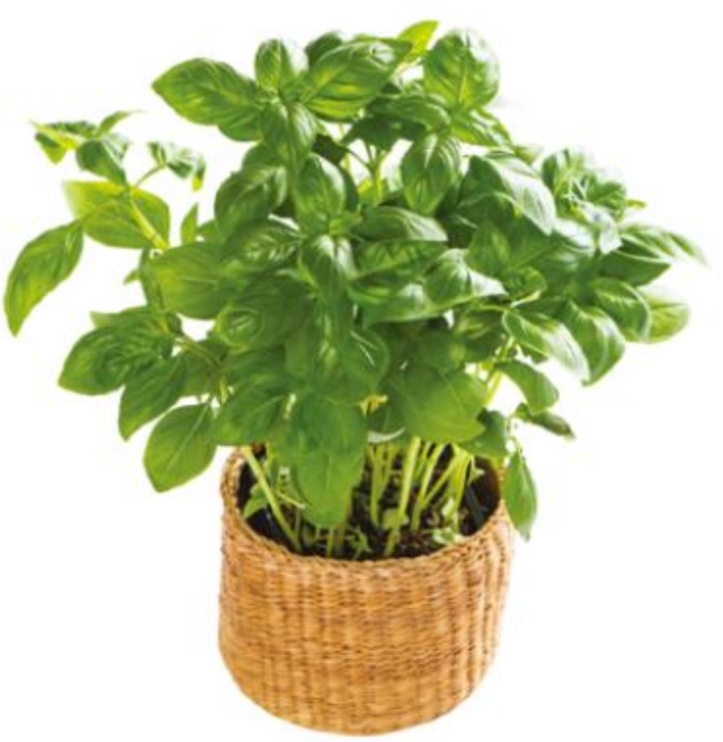
\includegraphics[scale=0.5]{Images/basilic.PNG}
        \end{center}
    \end{doc}
\end{minipage}
\begin{minipage}{0.5\textwidth}
\begin{doc}{Composition du basilic pour 100g}
     \begin{center}
        \begin{tabular}{|c|c|}
        \hline
             \cellcolor{blue!25} Espèces & \cellcolor{blue!25} Masse pour 100g  \\
        \hline
             Eau \chemform{H_2O} & 90,8g \\
        \hline
             Ion calcium \chemform{Ca^{2+}} & 273~mg\\
        \hline
             Acide oléique \chemform{C_{18}H_{34}O_2} & 0,09~g\\
        \hline
            Vitamine A \chemform{C_{20}H_{30}O} & 523~$\mu$g\\
        \hline 
            Autres & 8,84~g \\
        \hline
        \end{tabular}
    \end{center}
\end{doc}
\end{minipage}
\newpage
\begin{doc}{Détermination de la masse d'une molécule ou d'un ion polyatomique}
\vspace{-1.5cm}
    \begin{tcolorbox}[colback=red!5!white,colframe=red!75!black,title=\textbf{Règle sur les molécules et les ions polyatomiques : }]
\begin{itemize}[label=\textbullet, font=\large]
    \item La masse d'une molécule se calcule en faisant la somme des masses de chacun des atomes la constituant. Exemple pour le glucose de formule chimique \chemform{C_6H_{12}O_6} : 
        \begin{equation*}
            m(\text{\chemform{C_6H_{12}O_6}}) = 6\times m(C) + 12\times m(H) + 6\times m(O)
        \end{equation*}
    \item C'est la même règle pour déterminer la masse d'un ion polyatomique. Exemple pour l'ion sulfate de formule chimique \chemform{SO_4}$^{2-}$ :
        \begin{equation*}
            m(\text{\chemform{SO_4}$^{2-}$}) = 1\times m(S) + 4\times m(O)
        \end{equation*}
\end{itemize}
\end{tcolorbox}
\end{doc}
\begin{minipage}{0.4\textwidth}
    \begin{doc}{Masse de quelques entités chimiques}
\vspace{-1cm}
\begin{align*}
    m(\text{H}) &= 1,67\times10^{-27}~\text{kg} \\  m(\text{C}) &= 1,99\times10^{-26}~\text{kg} \\
    m(\text{O}) &= 2,66\times10^{-26}~\text{kg} \\ m(\text{Ca$^{2+}$}) &= 6,66\times10^{-26}~\text{kg} 
\end{align*}
\end{doc}
\end{minipage}
\begin{minipage}{0.6\textwidth}
\begin{doc}{Modèle moléculaire de l'acide oléique}
\vspace{-1cm}
\begin{center}
    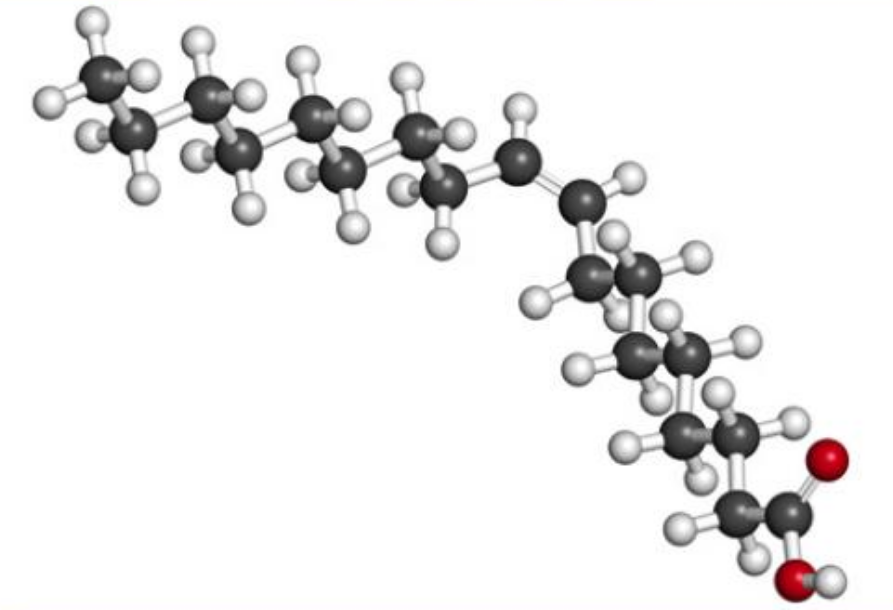
\includegraphics[scale=0.4]{Images/Modele_moleculaire_acideoleique.PNG}
\end{center}
\end{doc}    
\end{minipage}
\vspace{0.5cm}
\renewcommand{\arraystretch}{1.5}
\question{\`{A} l'aide du document 2, classer les quatre constituants du basilic donnés selon la nature des entités qui les constituent (atomique, ionique moléculaire) : 
\begin{center}
        \begin{tabular}{|C{0.31}|C{0.31}|C{0.31}|}
        \hline
             \cellcolor{orange!25} Atomique & \cellcolor{orange!25}Moléculaire & \cellcolor{orange!25} Ionique \\ 
            \hline
             & & \\
             \hline
        \end{tabular}
\end{center}
}
{\begin{center}
    \begin{tabular}{|C{0.31}|C{0.31}|C{0.31}|}
        \hline
        \cellcolor{orange!25} Atomique & \cellcolor{orange!25}Moléculaire & \cellcolor{orange!25} Ionique \\ 
        \hline
        & Eau, acide oléique, Vitamine A & Ion calcium Ca$^{2}$\\
        \hline
        \end{tabular}
\end{center}}{0}

\question{\`{A} l'aide du document 2 et 5, déterminer le nombre d'atomes de carbone, d'oxygène et d'hydrogène dans l'acide oléique. \newline\texteTrouMultiLignes{~}{3}}{Les indices correspondent aux nombre d'atomes présents dans la molécule : il y a donc 6 atomes de carbone, 34 atomes d'hydrogène et 2 atomes d'oxygène.}{0}
\\
\question{En vous aidant des règles du document 3, calculer la masse d'une seule entité pour chacune des espèces chimiques du basilic. \newline\texteTrouMultiLignes{~}{15}}{
\begin{itemize}
    \item Pour l'eau \chemform{H_2O} : $m(\text{\chemform{H_2O}})=m(O)+2\times m(H) = 1\times 2,66\times10^{-26} + 2\times 1,67\times10^{-27} = 2,99\times10^{-26}$~kg ;
    \item Pour l'ion calcium \chemform{Ca^+} : $m(\text{\chemform{Ca^{2+}}}) = m(Ca) = 6,66\times10^{-26}$~kg ;
    \item Pour l'acide oléique \chemform{C_{18}H_{34}O_2} :
    $m(\text{\chemform{C_{18}H_{34}O_2}}) = 18\times m(C) + 34\times m(H) + 2\times m(O) = 46,8\times10^{-26}$~kg ;
    \item Pour la vitamine A \chemform{C_{20}H_{30}O} : $m(\text{\chemform{C_{20}H_{30}O}}) = 20\times m(C) + 30\times m(H) + 2\times m(O) = 47,5\times10^{-26}$~kg ;
\end{itemize}
}{0}
%\\
\question{Déterminer le nombre de ces entités dans 100~g de basilic. \newline\texteTrouMultiLignes{~}{10}}{Le nombre d'une entité peut être calculé comme la masse totale de l'entité présente dans le basilic pour 100~g divisé par la masse d'une entité. Donc :
\begin{itemize}
    \item Pour l'eau \chemform{H_2O} : $N(\text{\chemform{H_2O}}) = \frac{m(\text{\chemform{H_2O},basilic})}{m(\text{\chemform{H_2O}})} = \frac{90,8\times10^{-3}~\text{kg}}{2,99\times10^{-26}~\text{kg}} = 30,4\times10^{23}$ molécules d'eau dans 100g de basilic ;
    \item Pour l'ion calcium \chemform{Ca^+} : $N(\text{\chemform{Ca^{2+}}}) = \frac{m(\text{\chemform{Ca^{2+}},basilic})}{m(\text{\chemform{Ca^{2+}}})} = 4,10\times10^{21}$ ions calcium dans 100g de basilic ;
    \item Pour l'acide oléique \chemform{C_{18}H_{34}O_2} :    $N(\text{\chemform{C_{18}H_{34}O_2}})= \frac{m(\text{\chemform{C_{18}H_{34}O_2},basilic})}{m(\text{\chemform{C_{18}H_{34}O_2}})} = 1,92\times10^{20}$ molécules d'acide oléique dans 100g de basilic ;
    \item Pour la vitamine A \chemform{C_{20}H_{30}O} : $N(\text{\chemform{C_{20}H_{30}O}}) = \frac{m(\text{\chemform{C_{20}H_{30}O},basilic})}{m(\text{\chemform{C_{20}H_{30}O}})} = 1,86\times10^{22}$ molécules de vitamine A dans 100g de basilic ;
\end{itemize}
}{0}


\begin{difficile}{Bilan de l'activité}
%\vspace{18cm}
Il existe une énorme quantité d'entités chimiques dans la matière à notre échelle ! Il est impossible de donner du sens à ces nombres pour le cerveau humain. D'autre part, le calcul est laborieux et relativement compliquer à réaliser.\\
Plutôt que de travailler avec les entités chimiques, le chimiste va plutôt les rassembler en \og paquets \fg~ d'un très grand nombre de particules. Un paquet est appelé \og \textcolor{red}{mole} \fg.\\
Soit N le nombre d'entités chimiques présentes et n le nombre de mole de cette entité présente dans une espèce chimique. Alors :
\begin{empheq}[box=\fbox]{equation*}
    \mathrm{N} = n\times\mathrm{N_A}
\end{empheq}
où :
\begin{empheq}[box=\fbox]{equation*}
    \mathrm{N_A} = 6,022\times10^{23}\text{mol$^{-1}$}
\end{empheq}
est appelé \textcolor{red}{constante d'Avogadro}. Cette constante représente le nombre d'entités chimiques par mole d'entité. Cette constante fait donc le lien entre l'échelle microscopique (l'entité) et l'échelle macroscopique (l'espèce chimique = collection d'un grand nombre d'entité).
\end{difficile}
  %%%%%%%%%% TP %%%%%%%%%%%%%%%
  %\modeCorrection

%%%% début de la page
\renewcommand{\thesection}{\textcolor{red}{Partie \Roman{section} -}}
\renewcommand{\thesubsection}{\textcolor{red}{\Roman{section}.\arabic{subsection}}}
\renewcommand{\thesubsubsection}{\textcolor{red}{\Roman{section}.\arabic{subsection}.\alph{subsubsection}}}

\setcounter{section}{0}
\setcounter{document}{0}
\sndEnTeteTPOnze

\begin{center}
\begin{mdframed}[style=titr, leftmargin=60pt, rightmargin=60pt, innertopmargin=7pt, innerbottommargin=7pt, innerrightmargin=8pt, innerleftmargin=8pt]

\begin{center}
\large{\textbf{TP 12 : \'{E}tude des composés ioniques
}}
\end{center}
\end{mdframed}
\end{center}


%%%% objectifs
\begin{tcolorbox}[colback=blue!5!white,colframe=blue!75!black,title=Objectifs de la séance :]
\begin{itemize}
    \item Mettre en œuvre des tests chimiques pour identifier des ions en solution  ;
    \item Exploiter l’électroneutralité de la matière pour associer des espèces ioniques et déterminer la formule d’un composé ionique ;
\end{itemize}
\end{tcolorbox}

%%%% Consignes
\begin{tcolorbox}[colback=red!5!white,colframe=red!75!black,title= Consignes :]
\begin{itemize}
    \item Faire attention au matériel lors de son utilisation ;
\end{itemize}
\end{tcolorbox}

%%%% contexte
\section{Analyse documentaire}
\begin{tcolorbox}[colback=orange!5!white,colframe=orange!75!black,title= Contexte : à quoi sert le nigari ? :]

\begin{minipage}{0.75\textwidth}
    Vous avez retrouvé dans votre cuisine un pot de nigari, un solide ionique naturel commercialisé sous forme de paillettes. Vous vous rappelez que ce nigari vous avez été recommandé pour les effets positifs qu'il pourrait avoir sur votre corps. Malheureusement, une partie de l’étiquette du pot de nigari s’est effacée et vous ne savez plus exactement pourquoi il vous avait été recommandé. 
\end{minipage}
\begin{minipage}{0.2\textwidth}
\begin{center}
    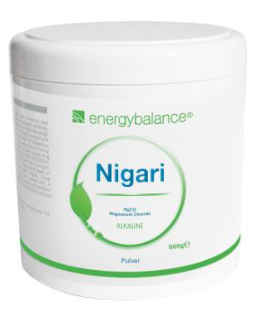
\includegraphics[scale=0.7]{Images/Nigari.PNG}
\end{center}
    
\end{minipage}

\problematique{Comment retrouver les bienfaits du nigari pour la santé ?}
\end{tcolorbox}


\begin{mdframed}[style=autreexo]
\textbf{\bsc{Liste du matériel}}
\vspace{-0.5cm}
\begin{multicols}{2}
\begin{itemize}
    \item Des paillettes de nigari ;
    \item Une solution d'oxalate d'ammonium ;
    \item Une solution d'hydroxyde de sodium ;
    \item Une solution de nitrate d'argent ;
    \item Une pissette d'eau distillée ; 
    \item Une spatule ;
    \item Des tubes à essais ;
\end{itemize}
\end{multicols}
\end{mdframed}
\clearpage

%%%% documents
\begin{doc}{Applications de quelques ions}
\vspace{-0.8cm}
\begin{center}
    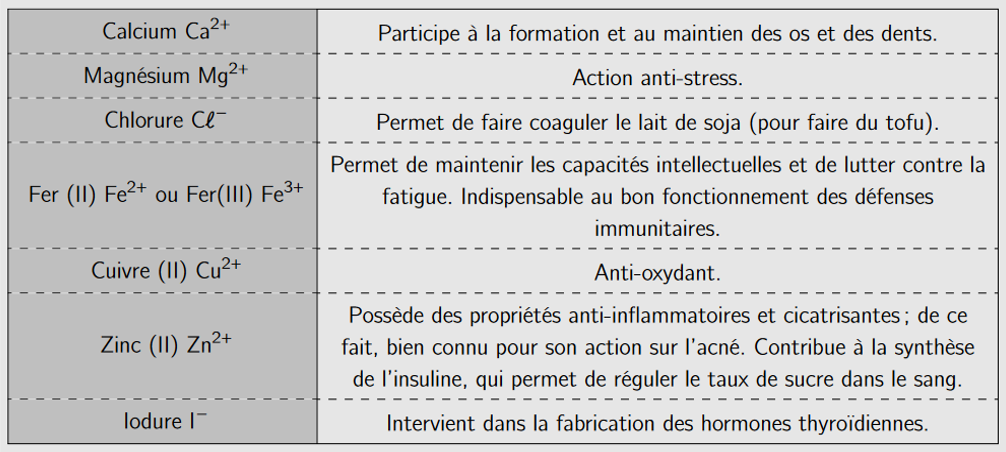
\includegraphics[scale=0.73]{Images/Ions.png}
\end{center}
\end{doc}

\begin{doc}{Identification de quelques ions}
\vspace{-0.8cm}
\begin{center}
    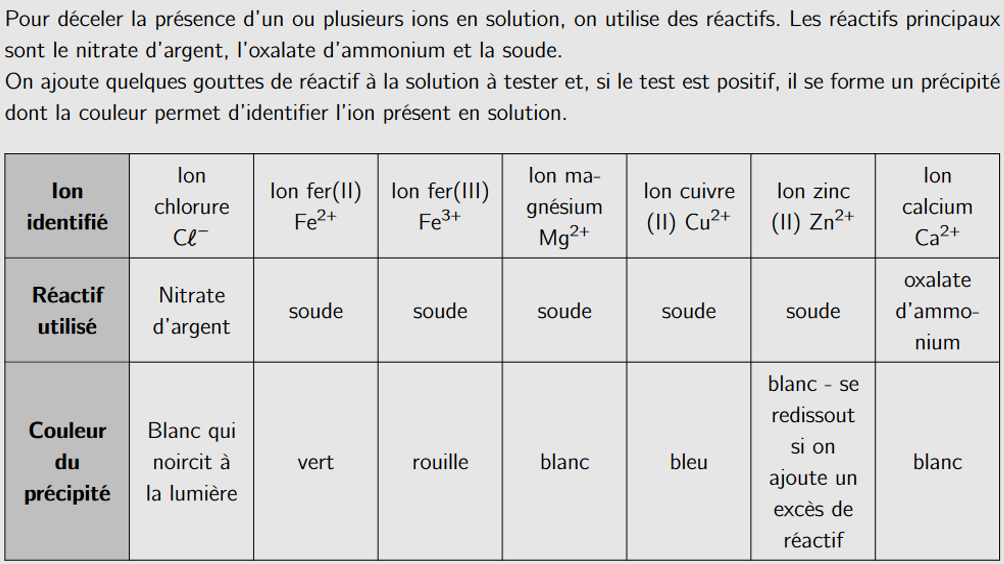
\includegraphics[scale=1]{Images/Ions_identification.png}
\end{center}
\end{doc}
\newpage
\begin{doc}{Définition et propriété d'un composé}
\vspace{-1cm}
\begin{center}
    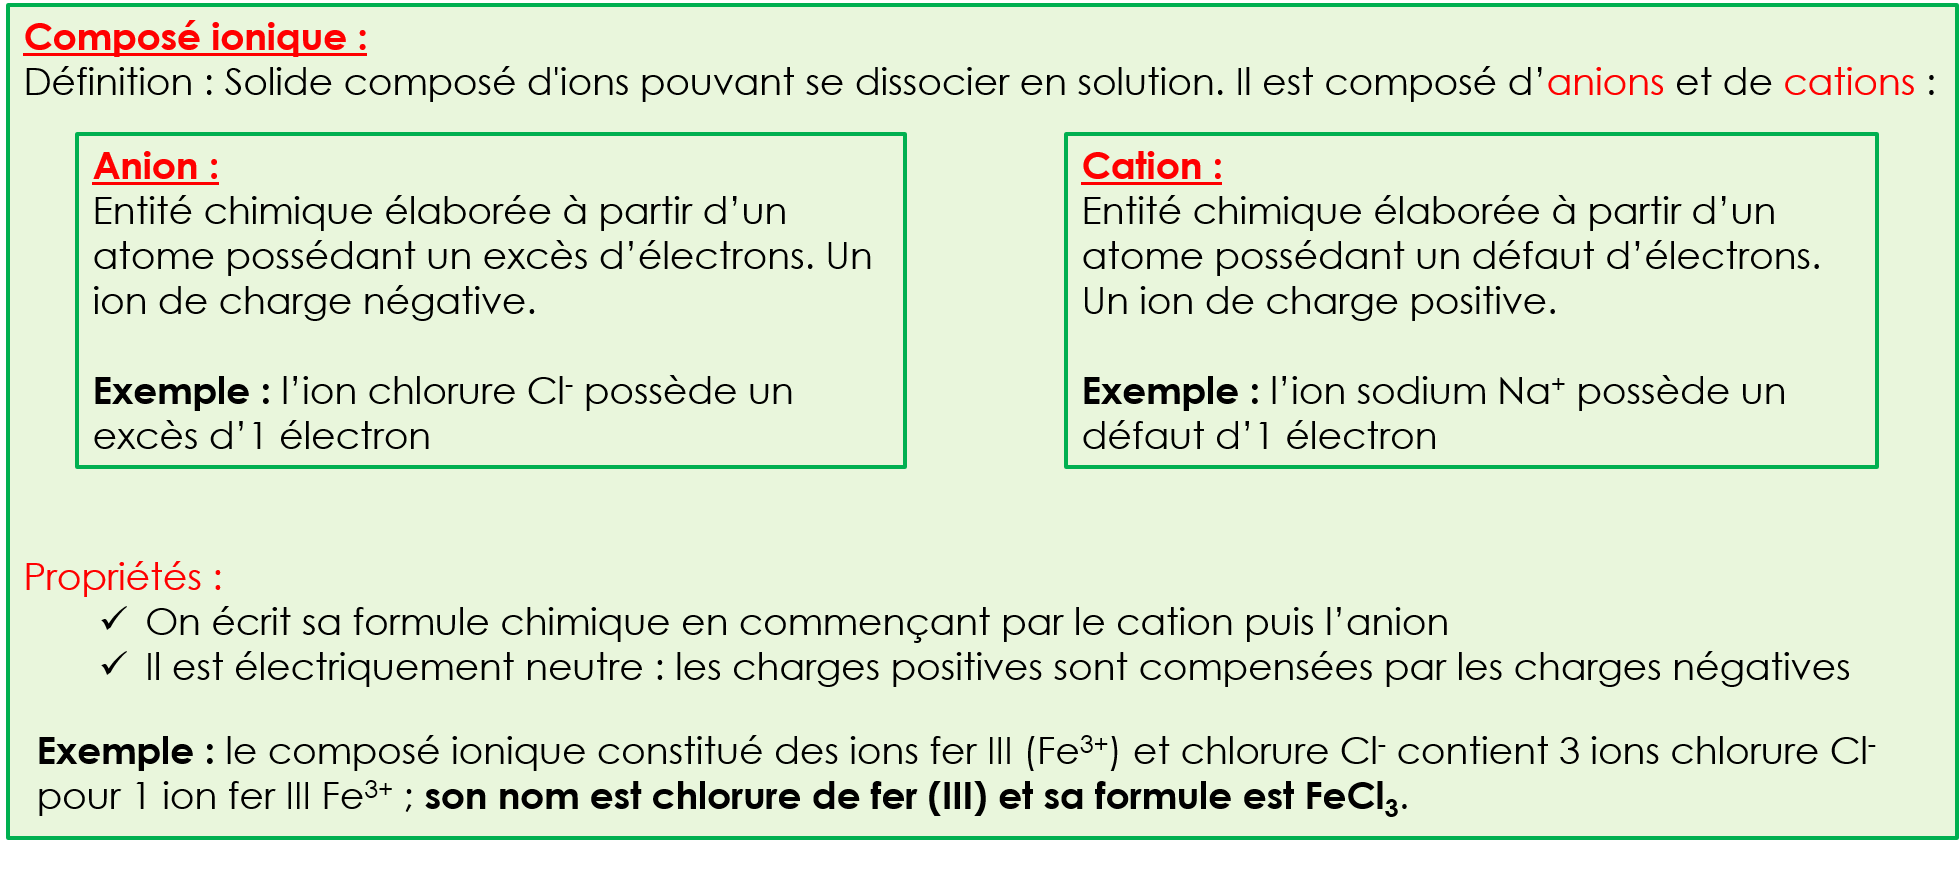
\includegraphics[scale=0.55]{Images/Solide_ionique.png}
\end{center}
\end{doc}

\question{Rappeler la problématique et proposer une hypothèse sur la nature des ions constituants le nigari.}{~}{0}
%\\
\question{Proposer un protocole expérimental permettant d’identifier les ions présents dans le Nigari. Vous pourrez utiliser des schémas accompagnés de phrases explicatives.}{~}{0}

\begin{center}
\begin{mdframed}[style=titr, leftmargin=60pt, rightmargin=60pt, innertopmargin=7pt, innerbottommargin=7pt, innerrightmargin=8pt, innerleftmargin=8pt]

\begin{center}
\begin{Large}
    \textcolor{red}{Appeler le professeur pour vérifier votre protocole.}
\end{Large}
\end{center}
\end{mdframed}
\end{center}

%\\
\question{Mettre en œuvre le protocole expérimental précédent.}{}{0}
%\\
\question{Noter vos observations.}{~}{0}
%\\
\question{Interprétations : en déduire les ions présents dans le nigari.}{~}{0}
%\\
\question{Conclusion : à l'aide du document 3, en déduire le nom et la formule du composé ionique constituant le nigari. Indiquer les effets bénéfiques et applications du nigari.}{~}{0}
\newpage

\begin{difficile}{Bilan à retenir}
\vspace{0.5cm}
\begin{multicols}{2}
\begin{center}
    On aurait pu tout faire à l'aide de ce logiciel de simulation (merci l'université du Colorado !) :

    \url{https://phet.colorado.edu/fr/simulations/geometric-optics-basics}\\
    \vspace{4cm}
    \begin{Large}
        \textbf{Mais c'est quand même bien mieux d'expérimenter en TP, non ??}
    \end{Large}
\end{center}

%\begin{center}
 %   \includegraphics[scale=0.15]{Images/Joyeux_noel_dispersé.png}
%\end{center}
\end{multicols}


\end{difficile}
%\newpage
%\papiermillimetre
  

  %%%%%%%%%% Devoirs Notés %%%%%%%%%%
  

\end{document}